% Every Latex document starts with a documentclass command
\documentclass[a4paper, 11pt]{article}

% Load some packages
\usepackage{graphicx} % This allows you to put figures in
\usepackage{natbib}   % This allows for relatively pain-free reference lists
\usepackage[left=2cm,top=3cm,right=2cm]{geometry} % The way I like the margins
\usepackage{framed}

\newcommand{\dnest}{{\tt DNest3}}

% This helps with figure placement
\renewcommand{\topfraction}{0.85}
\renewcommand{\textfraction}{0.1}
\parindent=0cm

% Set values so you can have a title
\title{{\tt DNest3} Manual}
\author{Brendon J. Brewer}
\date{\today}

% Document starts here
\begin{document}

% Actually put the title in
\maketitle

\section{Introduction}

\dnest~is a multi-threaded C++ implementation of Diffusive Nested Sampling, a
powerful Markov Chain Monte Carlo (MCMC) algorithm that is mainly
useful for solving Bayesian Inference problems.
\dnest~is free software,
released under the terms of the GNU General Public Licence, version 3.
For information about how the
algorithm works, please see the paper, freely available from the following
URL:\\

\begin{center}
{\tt http://arxiv.org/abs/0912.238}
\end{center}

If you find \dnest~useful, please feel free to cite the paper.
Throughout this manual I will assume that you have read the paper and have a
reasonable understanding of how the algorithm works, as well as some
understanding of Nested Sampling in general, as introduced by John Skilling.\\

\section{Installation}
Please note that I have only ever compiled \dnest~on GNU/Linux,
using the GNU C++ compiler ({\tt g++}). However, I expect it to be
straightforward to compile it on any other Unix-like operating system such as Mac
OS X or FreeBSD. It should be possible, albeit probably more tricky,
to compile \dnest~in Microsoft Windows. If you want to try,
the MinGW compiler is
probably your best bet. I'd be interested to hear from anyone who
has tried this. I would also be interested to hear if anyone has
compiled \dnest~with a different compiler, such as the Intel C++
compiler.\\

\subsection{Dependencies}
\dnest~depends on some other software that you will need to have installed on
your system. These should be quite easy to obtain. I highly
recommend obtaining these programs from your operating system's package manager,
rather than installing them from the source code. Note that some OSs split up
packages into binaries (the library files) and ``development'' packages,
containing header files (part of a library's source code).
In Ubuntu, Linux Mint, and Debian, the development packages have a -dev suffix.
In Fedora, the development packages usually have a -devel suffix (e.g. Fedora).
To compile \dnest, you will need both the libraries and the development packages
for each of the dependencies. Here's a list of dependencies:\\

\begin{itemize}
\item The GNU Scientific Library (GSL)
\item Python 2, along with the NumPy and matplotlib packages
\item The {\tt thread} and {\tt system} parts of the Boost C++ library.
It may be easier to just install all of Boost.
\item To compile \dnest, you need {\tt cmake}.\\
\end{itemize}

On Ubuntu, I can install these packages with the following commands:
\begin{verbatim}
sudo apt-get install libgsl0-dev
sudo apt-get install python-numpy python-matplotlib
sudo apt-get install libboost-thread-dev libboost-system-dev
sudo apt-get install cmake
\end{verbatim}

\dnest~uses GSL's random number generator. Python, NumPy and
matplotlib are used for the postprocessing scripts and for
plotting. Boost is used for parallelization (multithreading).
While random number generation and
multithreading is supported
in the recent C++11 standard, I have not ported \dnest~to C++11 and have no
intention of doing so in the near future.\\

It is also possible to compile \dnest~without Boost, however this is not
recommended, and you will not be able to use any of the multi-threaded options.\\

\subsection{Compiling}
Please follow the instructions in README.md to compile \dnest3~using cmake.
This is the recommended option.\\

%Go into the \dnest~directory and type {\tt make}. Everything should compile.
To
verify that the compilation was successful,
go into the {\tt Examples/SpikeSlab} directory
and see if an executable file called {\tt main} has been created. If you
execute this file, you should see a lot of output about ``levels'' and
``particles'' (see Figure~\ref{fig:output} for example output).
You will need to manually terminate this process by using
Control+C, or whatever works in your operating system. If you saw this output,
\dnest~was compiled successfully.\\

\section{Running DNest}
As part of the compilation process, several examples will have been compiled.
There is one executable file for each example: \dnest3 does not have a global
executable. The
following discussion will involve running the ``SpikeSlab'' example, which is
the example used in the paper.\\

To run the SpikeSlab example, go into the {\tt Examples/Spikeslab}
directory and execute {\tt main}. You should see some output that looks like
that shown in Figure~\ref{fig:output}.
Note that you must terminate the process manually by pressing Ctrl+C
or in another way. If you do not terminate the process yourself, it will run
forever. There is no definite rule for how long you should run \dnest.
It depends on the difficulty of your problem, the number of posterior samples you
want, and the accuracy you want for the marginal likelihood.\\

\begin{figure}[h!]
\begin{framed}
\begin{verbatim}
$ ./main
# Using 1 thread.
# Target compression factor between levels = 2.7182818284590451
# Seeding random number generator with 1402801184.
# Thread 1: Generated 1 particles from the prior.
# Creating level 1 with logL = -51.65058877.
# Creating level 2 with logL = -37.67550971.
# Creating level 3 with logL = -28.69668897.
# Creating level 4 with logL = -21.61338509.
# Creating level 5 with logL = -15.92331209.
# Creating level 6 with logL = -11.291182.
# Saving a particle to disk. N = 1.
# Creating level 7 with logL = -7.301954778.
# Creating level 8 with logL = -4.116771404.
# Creating level 9 with logL = -1.19393518.
# Creating level 10 with logL = 1.620392784.
# Saving a particle to disk. N = 2.
\end{verbatim}
\end{framed}
\caption{\it An example of \dnest~output that is shown on the screen. More
detailed information is saved to the three output files
{\tt sample.txt}, {\tt sample\_info.txt}, and {\tt levels.txt}.
\label{fig:output}}
\end{figure}

The executable {\tt main} is responsible for the exploration part of the
Diffusive Nested Sampling algorithm (i.e. running the MCMC chain, building
levels, and then exploring all the levels). It creates three output text files,
{\tt sample.txt}, {\tt sample\_info.txt}, and {\tt levels.txt}.\\

The first output
file, {\tt sample.txt}, contains a sampling of parameter values that
represents the {\it mixture of constrained priors} (the target distribution
used in Diffusive Nested Sampling), {\bf not} the
posterior distribution. Each line of {\tt sample.txt} represents a point in
parameter space. In the SpikeSlab example, there are 20 parameters, so there
will be 20 columns in {\tt sample.txt}.
Each time a point is saved to {\tt sample.txt}, \dnest~prints
the message ``Saving a particle to disk. N = ...''.\\

The second output file, {\tt sample\_info.txt}, should have the same number of
rows as {\tt sample.txt}, because it contains metadata about the samples in
{\tt sample.txt}. The first
column is the index $j$, which tells us which ``level'' the particle was in
when it was saved. Level 0 represents the prior, and higher levels represent
more constrained versions of the prior.
The second column is the log-likelihood value, and the third column is
the likelihood ``tiebreaker'', which allows Nested Sampling to work when
there is a region in parameter space with nonzero prior probability where the
likelihood is constant. The final column tells us which thread the particle
belonged to: when you use \dnest~in multithreaded mode, each thread
is responsible for evolving one or more walkers.\\

The third output file, {\tt levels.txt}, contains information about the levels
that were built during the run. The first column has estimates of the $\log(X)$
values of the levels, i.e. how compressed they are relative to the prior, in
units of nats. The second column contains the log likelihoods of the levels.
The first level, with a $\log(X)$ value of 0 and a log likelihood of
$-10^{300}$ (basically ``minus infinity''), is simply the prior. The third
column has the ``tiebreaker'' values for the levels, which again are not
particularly useful unless your problem has likelihood plateaus. The fourth
and fifth columns are the number of accepted proposals and the total number
of proposals that have occurred within each level, which are useful for
monitoring the Metropolis acceptance ratio as a function of level.
The final two columns, called ``exceeds'', and ``visits'', are used to refine
the estimates of the level compressions (and hence the $\log(X)$ values of
the levels in column 1), as discussed in Section 3 of the
paper. The visits column counts the number of times a level (level $j$, say)
has been visited, but only starts counting after the next level ($j+1$) has been created. The exceeds column counts the number of times a particle that was
in level $j$ had a likelihood that exceeded that of level $j+1$.
\\

\section{Postprocessing with showresults.py}
After {\tt main} has been running for
a while, you should run the postprocessing script
by executing {\tt python showresults.py}. This script loads the output files,
plots some graphs, and creates two new output files, {\tt weights.txt} and
{\tt posterior\_samples.txt}. It also prints the current estimate of the
(log of the) marginal likelihood or evidence value (traditionally considered
the main goal of Nested Sampling), as well as the information value (the KL
divergence from the prior to the posterior).\\

The plots made by {\tt showresults.py} are conceptually similar to plots in
the DNS paper. The first plot shows the level of the saved particles vs.
time, the equivalent of Figure 2 in the paper. The second plot produced by
{\tt showresults.py} shows the estimated compression values of the levels,
like in Figure 3 of the paper, along with the Metropolis acceptance fraction
as a function of the level (as you would expect, this usually shows a
decreasing trend). The final plot corresponds to Figure 4 from the paper, and
shows the shape of the likelihood curve along with the posterior weights of
the saved particles.\\

The plots are useful to diagnose the progress of your run. For example, you
want to ensure that the Metropolis acceptance fraction doesn't drop to near
zero. If it does, the proposal distributions might be too aggressive, or maybe
you just created too many levels (and the high level distributions are just
extremely narrow). The other key plot for diagnostics is the posterior
weights. On most problems, these will peak at some point, and begin to
come back down towards zero. Once this occurs, you probably have enough levels.
It is wasteful to create large amounts of levels extending well beyond the peak.
However, on problems with phase transitions more than one peak may occur.\\

\begin{figure}
\begin{center}
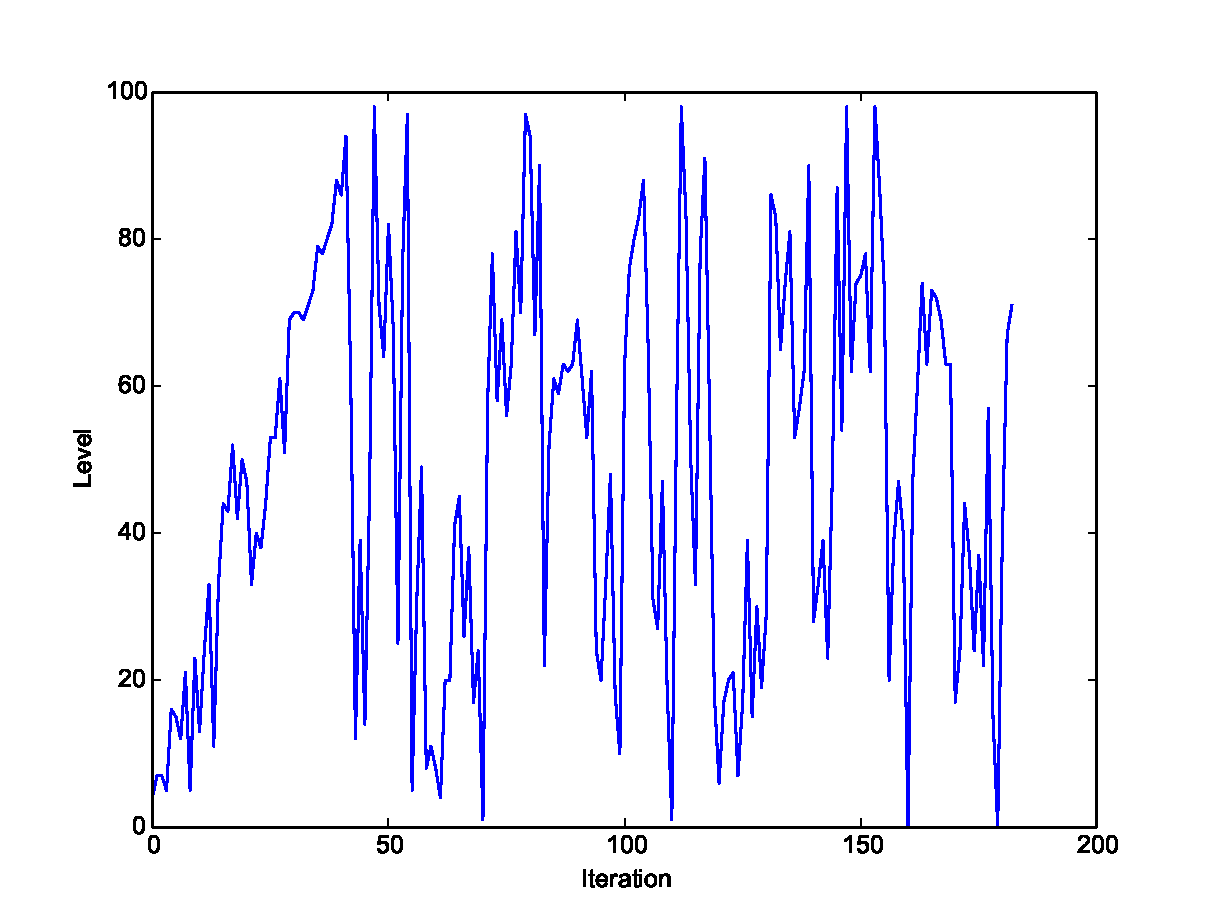
\includegraphics[scale=0.5]{fig1.pdf}
\caption{\label{fig:fig1}}
\end{center}
\end{figure}

\begin{figure}
\begin{center}
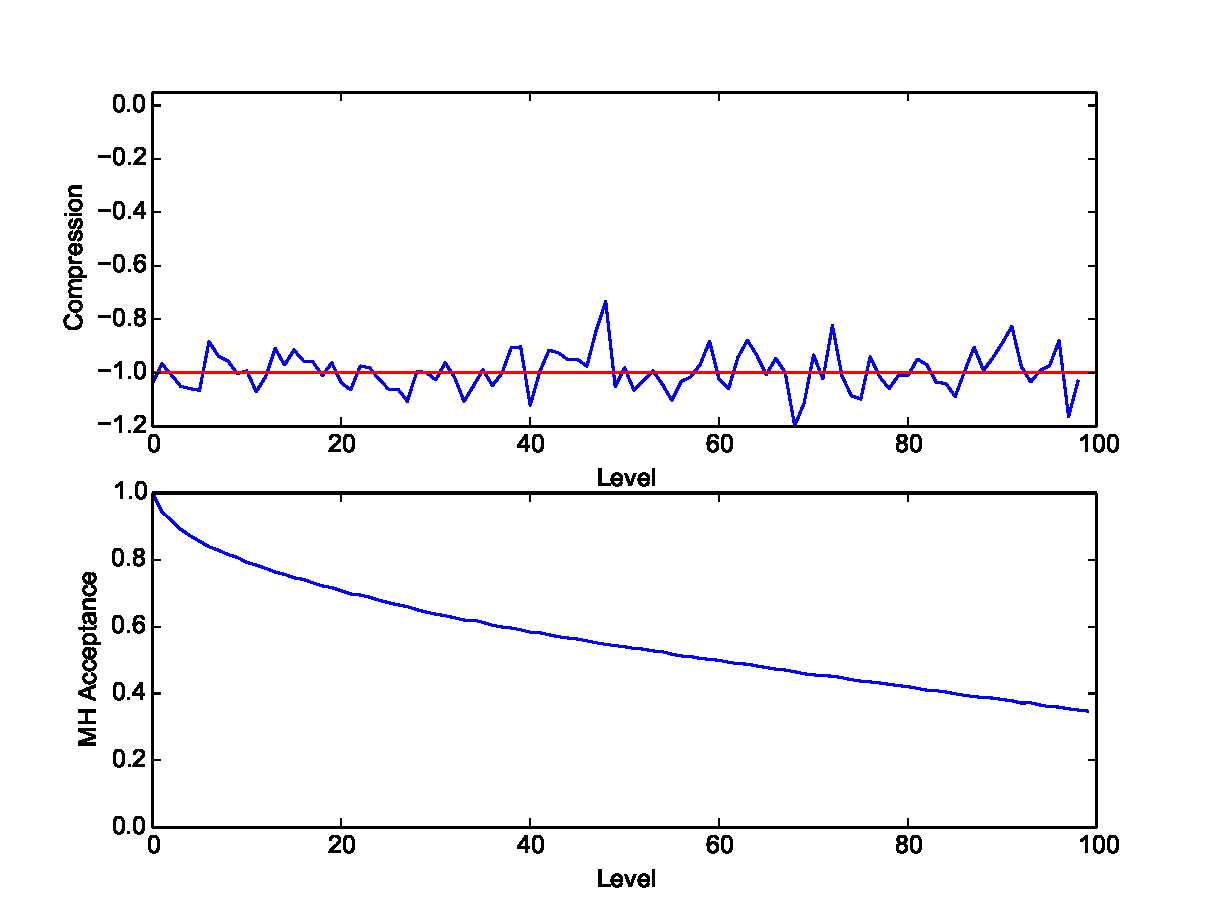
\includegraphics[scale=0.5]{fig2.pdf}
\caption{\label{fig:fig2}}
\end{center}
\end{figure}

\begin{figure}
\begin{center}
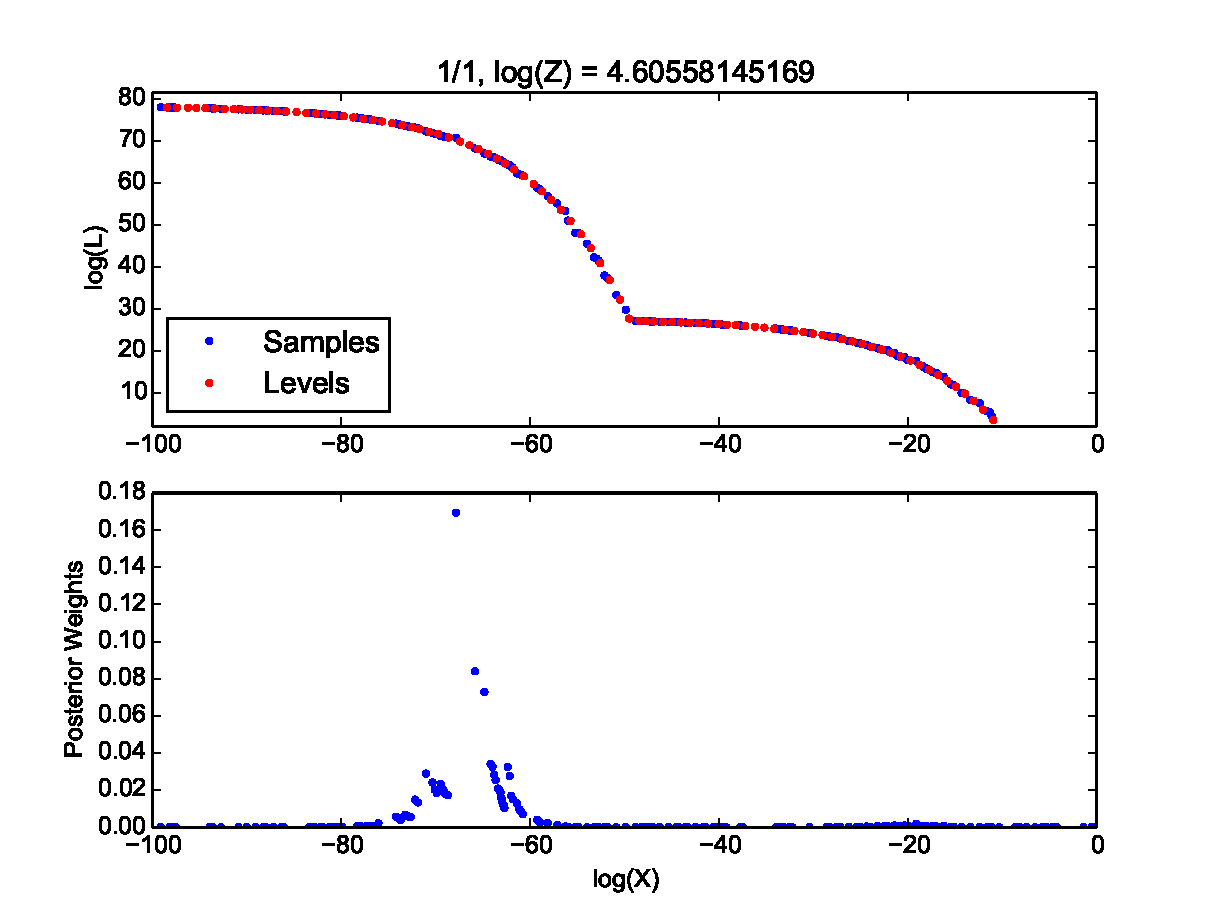
\includegraphics[scale=0.5]{fig3.pdf}
\caption{\label{fig:fig3}}
\end{center}
\end{figure}

\section{Command line options}
\dnest~executables allow for several command line options. A couple of these
options are quite important, while others are much less useful.
You can view the available options by executing
{\tt ./main -h}. Here is the list:\\

\begin{verbatim}
DNest3 Command Line Options:
-h: display this message
-l <filename>: load level structure from the specified file.
-o <filename>: load DNest3 options from the specified file. Default=OPTIONS
-s <seed>: seed the random number generator with the specified value.
           If unspecified, the system time is used.
-d <filename>: Load data from the specified file, if required.
-c <value>: Specify a compression value (between levels) other than e.
-t <num_threads>: run on the specified number of threads. Default=1.
\end{verbatim}
The most important option is the one about the number of threads. Depending on
your computer, you probably want to run \dnest~with more than one thread.
Each thread will be responsible for evolving its own walker(s), and periodically
the threads will pool their results (for example, information about the
levels). To execute DNest with 8 threads, simply use {\tt ./main -t 8}. You can
replace 8 with however many threads you want. I usually use 8 threads because
that's how many my computer can run simultaneously at full speed.\\

In many Monte Carlo studies, it is useful to be able to set the random number
seed, for debugging and reproducibility reasons. By default \dnest~seeds the
random number generator with the system time, and displays the value of the
seed in the output (you can see this in the example output displayed above).
If you want to set the seed to
something else, use the {\tt -s} option and specify a non-negative integer for
the seed. For example, to execute \dnest~with
8 threads and a seed of 42, use {\tt ./main -t 8 -s 42}.
When running with multiple threads, \dnest~uses a separate generator for each
thread, and ensures that they are seeded with different values.\\

\section{The OPTIONS file}
Here is an example OPTIONS file.
\begin{verbatim}
1	# Number of particles
10000	# new level interval
100000	# save interval
200	# threadSteps
100	# maximum number of levels
10	# Backtracking scale length (lambda in the paper)
10	# Strength of effect to force histogram to equal push. (beta in the paper)
0	# Maximum number of saves (0 = infinite)
\end{verbatim}
The first option is the number of particles {\it per thread}. If you run
\dnest~with 8 threads, there will actually be 8 particles. For most
applications, 1 particle per thread is sufficient. If you use more particles
per thread, the same amount of CPU time will be spent evolving more particles,
so each one will not be evolved as far. On most problems, one particle per
thread is fine. I would only use more particles per thread when working on
a very hard problem where it is difficult for the particles to find the
important parts of parameter space.\\

The new level interval controls how quickly \dnest~creates new levels. In this
example, this is set to 10,000, so a new level will be created once \dnest~has
seen 10,000 likelihood values above the current top level. This is not affected by
the number of threads. It is difficult to give a sensible default for this
quantity because it depends on the complexity of the problem and how good
the Metropolis proposals are. However, 10,000
will work for many problems (I rarely use anything less than 10,000 or greater
than 300,000). Higher values are slower, but more fail-safe.\\

%    <h3>Compiling<br>
%    </h3>
%    To compile DNest3, simply run<br>
%    <br>
%    <span style="font-family: monospace;">make</span><br>
%    <br>
%    in the root DNest3 directory. This will create <span
%      style="font-family: monospace;"></span>a static library <span
%      style="font-family: monospace;">libdnest3.a</span> in the current
%    directory. If you like, feel free to copy these to some other
%    location on your system, for example <span style="font-family:
%      monospace;">/usr/local/lib</span>. It will also compile the
%    examples in the <span style="font-family: monospace;">Examples/</span>
%    directory, creating executable files called <span
%      style="font-family: monospace;">main</span> that you can use to
%    run the examples.<br>
%    <h3>Running the Examples</h3>
%    Two examples are provided with DNest3. I will now explain how DNest3
%    is used through the first example, <span style="font-style:
%      italic;">SpikeSlab</span>.<br>
%    <h4>Example 1: SpikeSlab</h4>
%    The first example, called <span style="font-style: italic;">SpikeSlab</span>,
%    is the demo problem from our <a
%      href="http://arxiv.org/abs/0912.2380">paper</a>, and is a slight
%    modification of one of the examples in <a
%href="http://citeseerx.ist.psu.edu/viewdoc/download?doi=10.1.1.117.5542&amp;rep=rep1&amp;type=pdf">John










%      Skilling's Nested Sampling Paper</a>. It is a problem with 20
%    unknown parameters, each with a uniform prior between -0.5 and 0.5.
%    The priors for all of the parameters are independent. The likelihood
%    function is a mixture of two Gaussians: one is a wide "slab" and the
%    other is a narrow "spike". The slab is centered at (0, 0, ..., 0)
%    with a width of 0.1 in each dimension. The spike is centered at
%    (0.031, 0.031, ..., 0.031) and has a width of 0.01 in each
%    dimension. This problem is challenging for all sampling algorithms
%    that are not variants of Nested Sampling.<br>
%    <br>
%    To run DNest3 on the <span style="font-style: italic;">SpikeSlab</span>
%    example, simply compile DNest3, then enter the SpikeSlab directory
%    and run <span style="font-family: monospace;">main</span>. <br>
%    <br>
%    <code><span style="font-family: monospace;">make<br>
%        cd Examples/SpikeSlab<br>
%        ./main</span></code><br style="font-family: monospace;">
%    <br>
%    You should see a bunch of output that looks like this:<br>
%    <samp><br>
%      # Using 1 thread.<br>
%      # Seeding random number generator with -1337625108.<br>
%      # Generating 3 particles from the prior...done.<br>
%      # Creating level 1 with logL = -51.91599704.<br>
%      # Creating level 2 with logL = -38.68866085.<br>
%      # Creating level 3 with logL = -29.30928837.<br>
%      # Creating level 4 with logL = -22.44227047.<br>
%      # Creating level 5 with logL = -16.947356.<br>
%      # Creating level 6 with logL = -12.19901323.<br>
%      # Saving a particle to disk. N = 1.<br>
%      # Creating level 7 with logL = -8.14478528.<br>
%      # Creating level 8 with logL = -4.640384951.<br>
%      # Creating level 9 with logL = -1.486986762.<br>
%      # Creating level 10 with logL = 1.317628374.<br>
%      # Saving a particle to disk. N = 2.<br>
%      # Creating level 11 with logL = 4.137860699.<br>
%      # Creating level 12 with logL = 6.379241865.<br>
%      # Creating level 13 with logL = 8.447578631.<br>
%      # Saving a particle to disk. N = 3.<br>
%      # Creating level 14 with logL = 10.09126447.<br>
%      # Creating level 15 with logL = 11.68745251.<span
%        style="font-family: monospace;"></span><br style="font-family:
%        monospace;">
%    </samp><br>
%    and so on. By default, this process will continue forever (this can
%    be overridden by using different OPTIONS). At some point, you should
%    kill it with Ctrl-C. Then, it is time to examine and process the
%    output. The executable itself creates the following output files:<br>
%    <br style="font-family: monospace;">
%    <span style="font-family: monospace;">levels.txt</span><br
%      style="font-family: monospace;">
%    <span style="font-family: monospace;">sample.txt</span><br
%      style="font-family: monospace;">
%    <span style="font-family: monospace;">sample_info.txt</span><br
%      style="font-family: monospace;">
%    <br>
%    Of these, <span style="font-family: monospace;">sample.txt</span>
%    is the most important file, as it contains the samples. Each line
%    corresponds to a sample, a point in the parameter space. However,
%    the samples in <span style="font-family: monospace;">sample.txt</span>
%    are <span style="font-style: italic;">not</span> posterior samples.
%    Instead, they are samples from the mixture distribution that DNest3
%    actually explores. To actually get posterior samples, you need to
%    run the post-processing script <span style="font-family:
%      monospace;">showresults.py</span>. This script produces useful
%    plots of the sort shown in the <a
%      href="http://arxiv.org/abs/0912.2380">paper</a>, and also creates
%    the following additional output files that will probably be of more
%    interest to you:<br>
%    <br>
%    <span style="font-family: monospace;">weights.txt</span><br
%      style="font-family: monospace;">
%    <span style="font-family: monospace;">posterior_sample.txt</span><span
%      style="font-family: monospace;"></span><br style="font-family:
%      monospace;">
%    <br>
%    The file <span style="font-family: monospace;">weights.txt</span>
%    contains importance weights for the samples in <span
%      style="font-family: monospace;">sample.txt</span>. Alternatively,
%    if you are not used to dealing with non-equally-weighted samples,
%    the file <span style="font-family: monospace;">posterior_sample.txt</span>
%    is for you!<br>
%    <br>
%    <span style="color: rgb(0, 0, 153);">Note: You can also run <span
%        style="font-family: monospace;">showresults.py</span> while the
%      main process is still running. In fact, this is recommended in any
%      non-trivial problem for monitoring the algorithm's progress. The
%      only issue is that the main process may write to the output files
%      while <span style="font-family: monospace;">showresults.py</span>
%      is trying to load them. This may case an "ERROR: Size mismatch"
%      message to be displayed. The workaround is to suspend the main
%      process with Ctrl-Z, run <span style="font-family: monospace;">showresults.py</span>
%      and then resume the main process with <span style="font-family:
%        monospace;">fg</span>.</span><span style="font-weight: bold;"><br>
%      <br>
%    </span>
%    <h3>Command-Line Options<br>
%    </h3>
%    Run <span style="color: rgb(0, 0, 153);"><span style="font-family:
%        monospace;">./main -h </span></span>to see a list of available
%    command-line options.<br>
%    <h3>TODO: Tuning the Numerical Parameters in 'OPTIONS'</h3>
%    <h3>TODO: Implementing your own Models</h3>
%    <h3>TODO: Tips and Tricks</h3>
%    <span style="font-family: serif;"> </span>
%    <h3>Other Recommended Samplers</h3>
%    While DNest3 is a very effective sampler and works on a wide range
%    of problems (including many problems with multi-modal posterior
%    distributions or strong correlations), there are a few situations
%    where I would recommend alternative methods. The primary situation
%    in which DNest3 is not recommended is where the calls to the
%    likelihood function are expensive, yet the number of parameters is
%    small to moderate.<br>
%    <br>
%    For these problems, I would recommend <a
%      href="http://github.com/dfm/emcee">emcee</a> in the case where
%    strong correlations may be present but multimodality is unlikely, or
%    <a href="http://ccpforge.cse.rl.ac.uk/gf/project/multinest/">MultiNest</a>
%    if multimodality is expected or if the value of the evidence
%    integral is required. These samplers also have the advantage of
%    requring less programming from the user. For example, emcee only
%    requires a likelihood function, whereas DNest3 requires that you
%    implement a likelihood function, a function to generate random
%    models from the prior, and a function for generating
%    Metropolis-Hastings proposals.<br>




\section{Running the examples}


\section{Writing your own models}



\end{document}

